\documentclass{article}

\usepackage{amsmath}
\usepackage{amsthm}
\usepackage{amssymb}
\usepackage{bbm}
\usepackage{fancyhdr}
\usepackage{float}
% \usepackage{listings}
\usepackage{cite}
\usepackage{graphicx}
\usepackage{enumitem}
\usepackage{courier}
\usepackage{caption}
\usepackage[pdftex,colorlinks=true, urlcolor = blue]{hyperref}

\usepackage{minted}

\oddsidemargin 0in \evensidemargin 0in
\topmargin -0.5in \headheight 0.25in \headsep 0.25in
\textwidth 6.5in \textheight 9in
\parskip 6pt \parindent 0in \footskip 20pt

% set the header up
\fancyhead{}
\fancyhead[L]{Stanford Aeronautics \& Astronautics}
\fancyhead[R]{Fall 2020}

%%%%%%%%%%%%%%%%%%%%%%%%%%
\renewcommand\headrulewidth{0.4pt}
\setlength\headheight{15pt}

\usepackage{xparse}
\NewDocumentCommand{\codeword}{v}{%
\texttt{\textcolor{blue}{#1}}%
}

\usepackage{xcolor}
\setlength{\parindent}{0in}

\title{AA 274A: Principles of Robot Autonomy I \\ Problem Set 4}
\author{Names: Parthiv Krishna, Shawn Manuel, Mason Llewellyn}
\date{}

\begin{document}

\maketitle
\pagestyle{fancy} 

\section*{Problem 1: EKF Localization}
\begin{enumerate}[label=(\roman*)]
\item Implemented \codeword{compute_dynamics()} in \codeword{turtlebot_model.py} and \codeword{transition_model()} in the \codeword{EKFLocalization} class in \codeword{ekf.py}.
\item Implemented the dynamics transition update in \codeword{transition_update()} in the \codeword{Ekf} class in \codeword{ekf.py}. Below is \codeword{ekf_open_loop.png}.

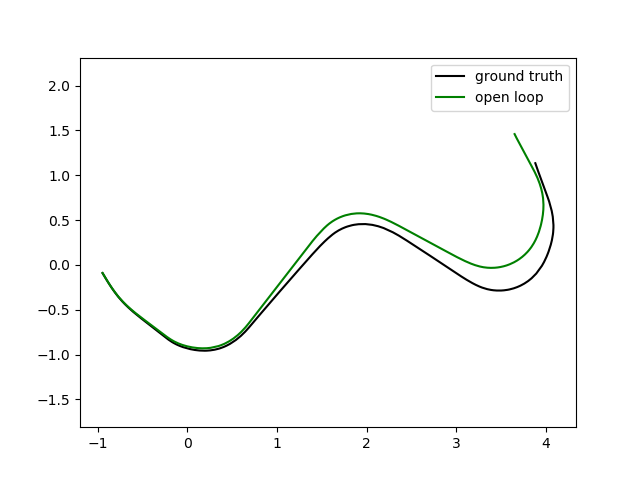
\includegraphics[width=\textwidth]{ekf_open_loop.png}

\item Implemented the coordinate change between the world frame and camera frame in \\ \codeword{transform_line_to_scanner_frame()} in \codeword{turtlebot_model.py}. Used this function to implement \codeword{compute_predicted_measurements()} in the \codeword{EkfLocalization} class in \codeword{ekf.py}.
\item Implemented the measurement association process in \codeword{compute_innovations()} in the \codeword{EkfLocalization} class in \codeword{ekf.py}.
\item Implemented \codeword{measurement_model()} in the \codeword{EkfLocalization} class in \codeword{ekf.py}.
\item Implemented \codeword{measurement_update()} in the \codeword{Ekf} class in \codeword{ekf.py}. Below is \\ \codeword{ekf_localization.png}. 

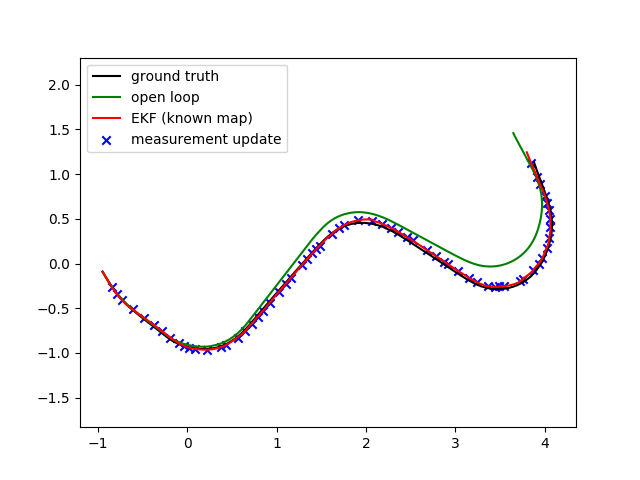
\includegraphics[width=\textwidth]{ekf_localization.png}

\item Copied the appropriate files to Genbu, launched \codeword{turtlebot3_maze.launch} and \\ \codeword{turtlebot3_teleop_key.launch}, and ran \codeword{localization.py}. 
\item It appears that the results diverge quite quickly when the robot rotates with high angular velocity. Since the update step takes some time, the rapidly changing heading of the robot presents a major challenge for associating measurements. Images are on the next page.

\newpage

\begin{figure}[H]
    \begin{center}
    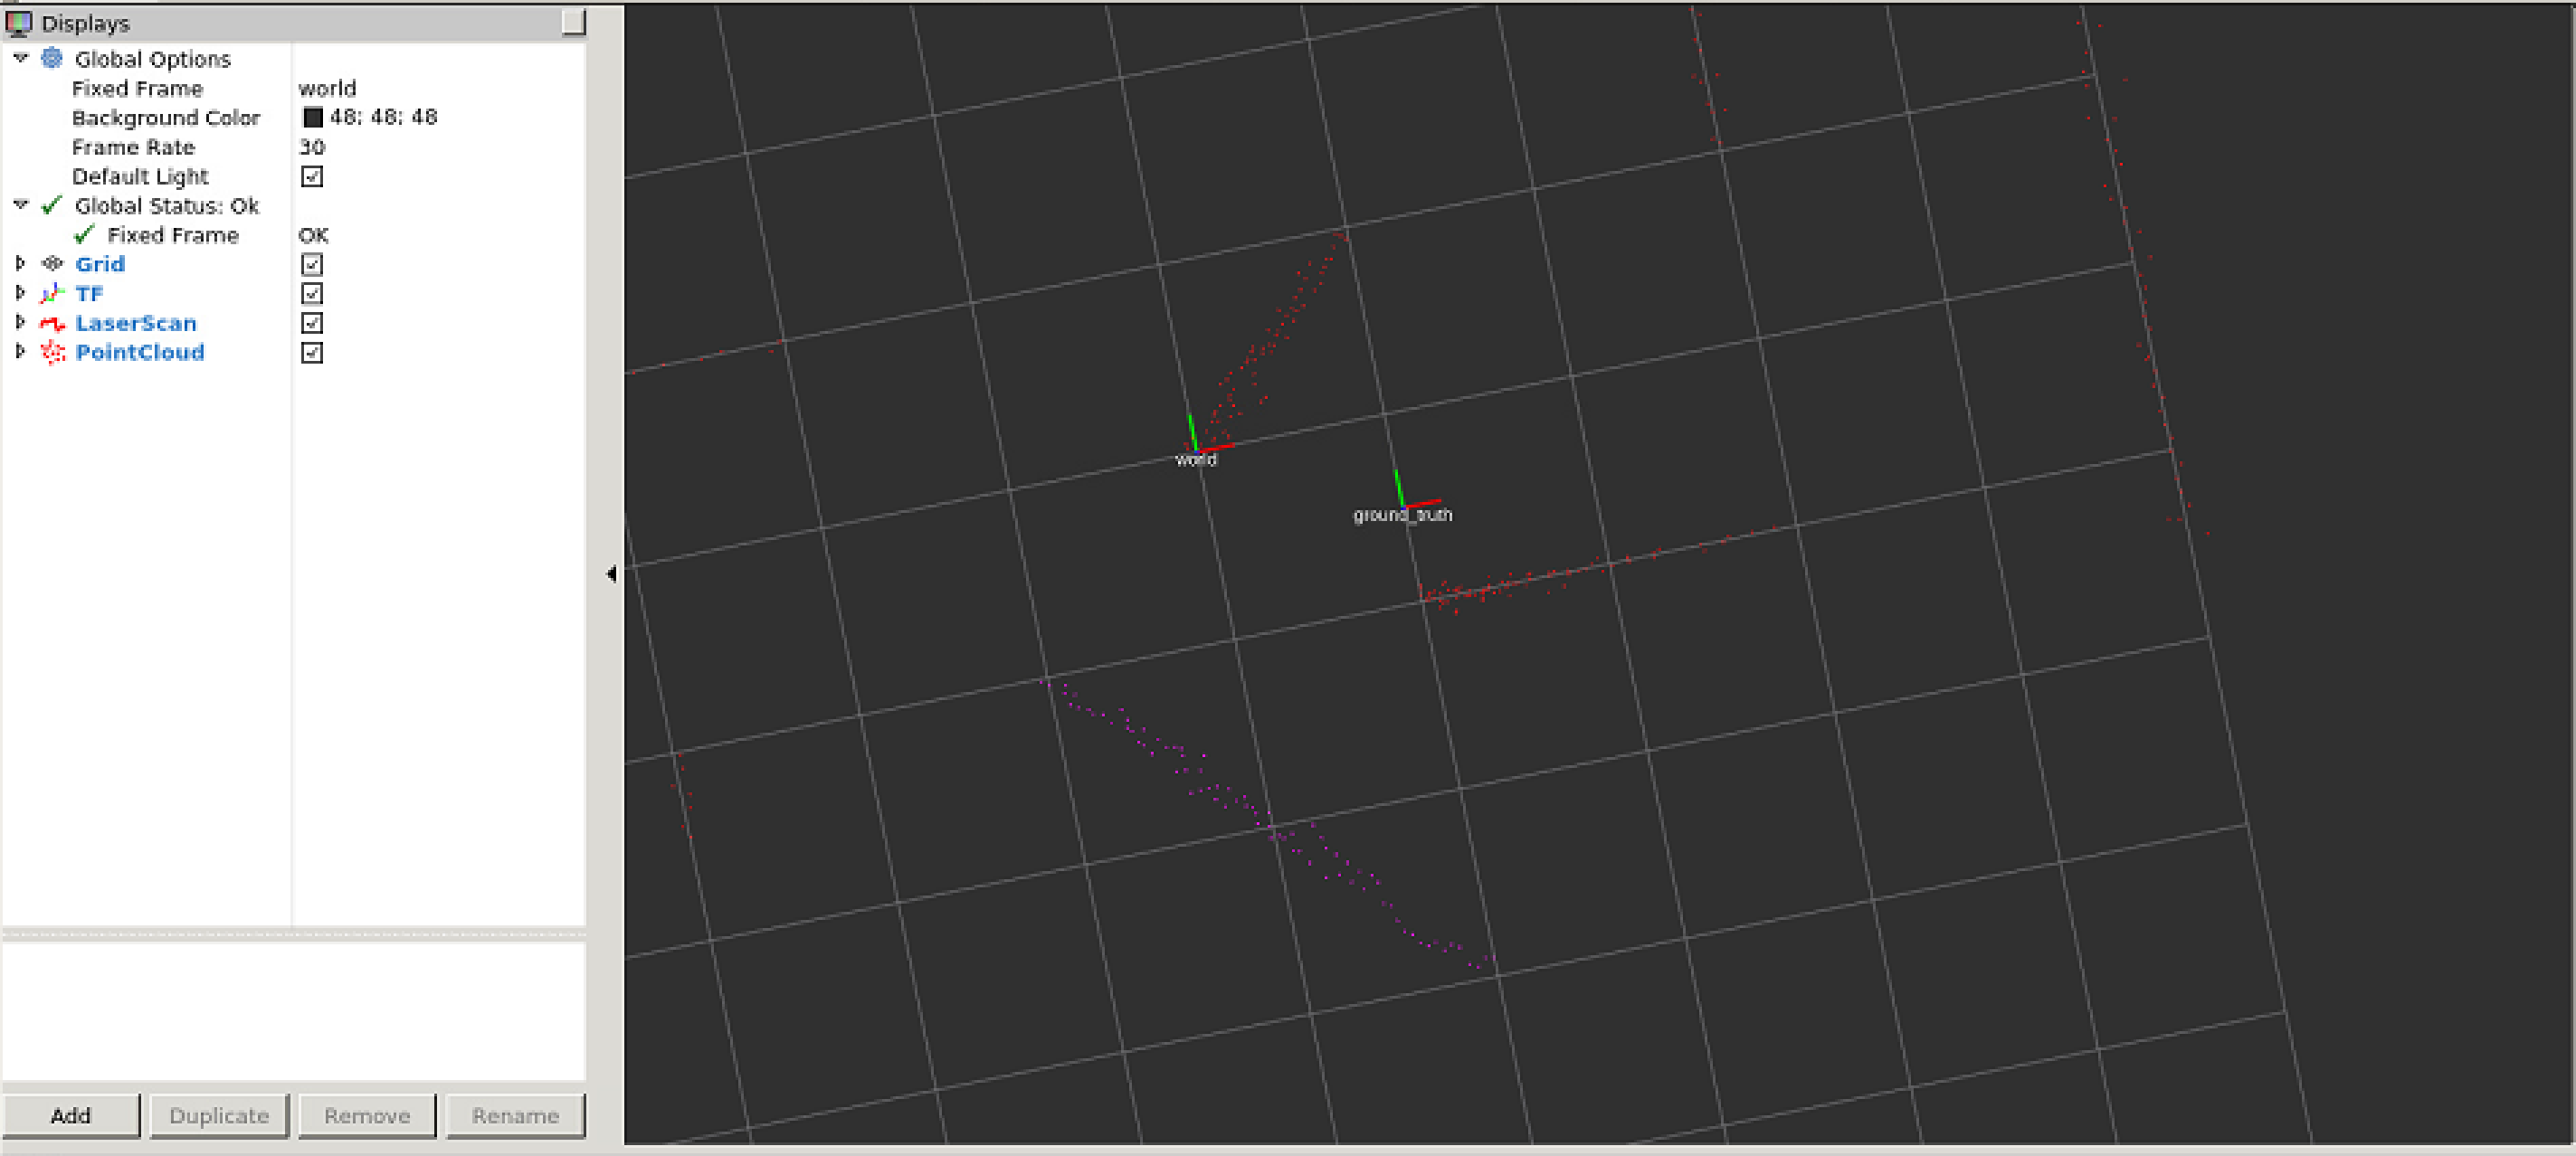
\includegraphics[width=0.65\textwidth]{P1_Screenshots/1initial.PNG}
    \caption*{(1) The initial state}
    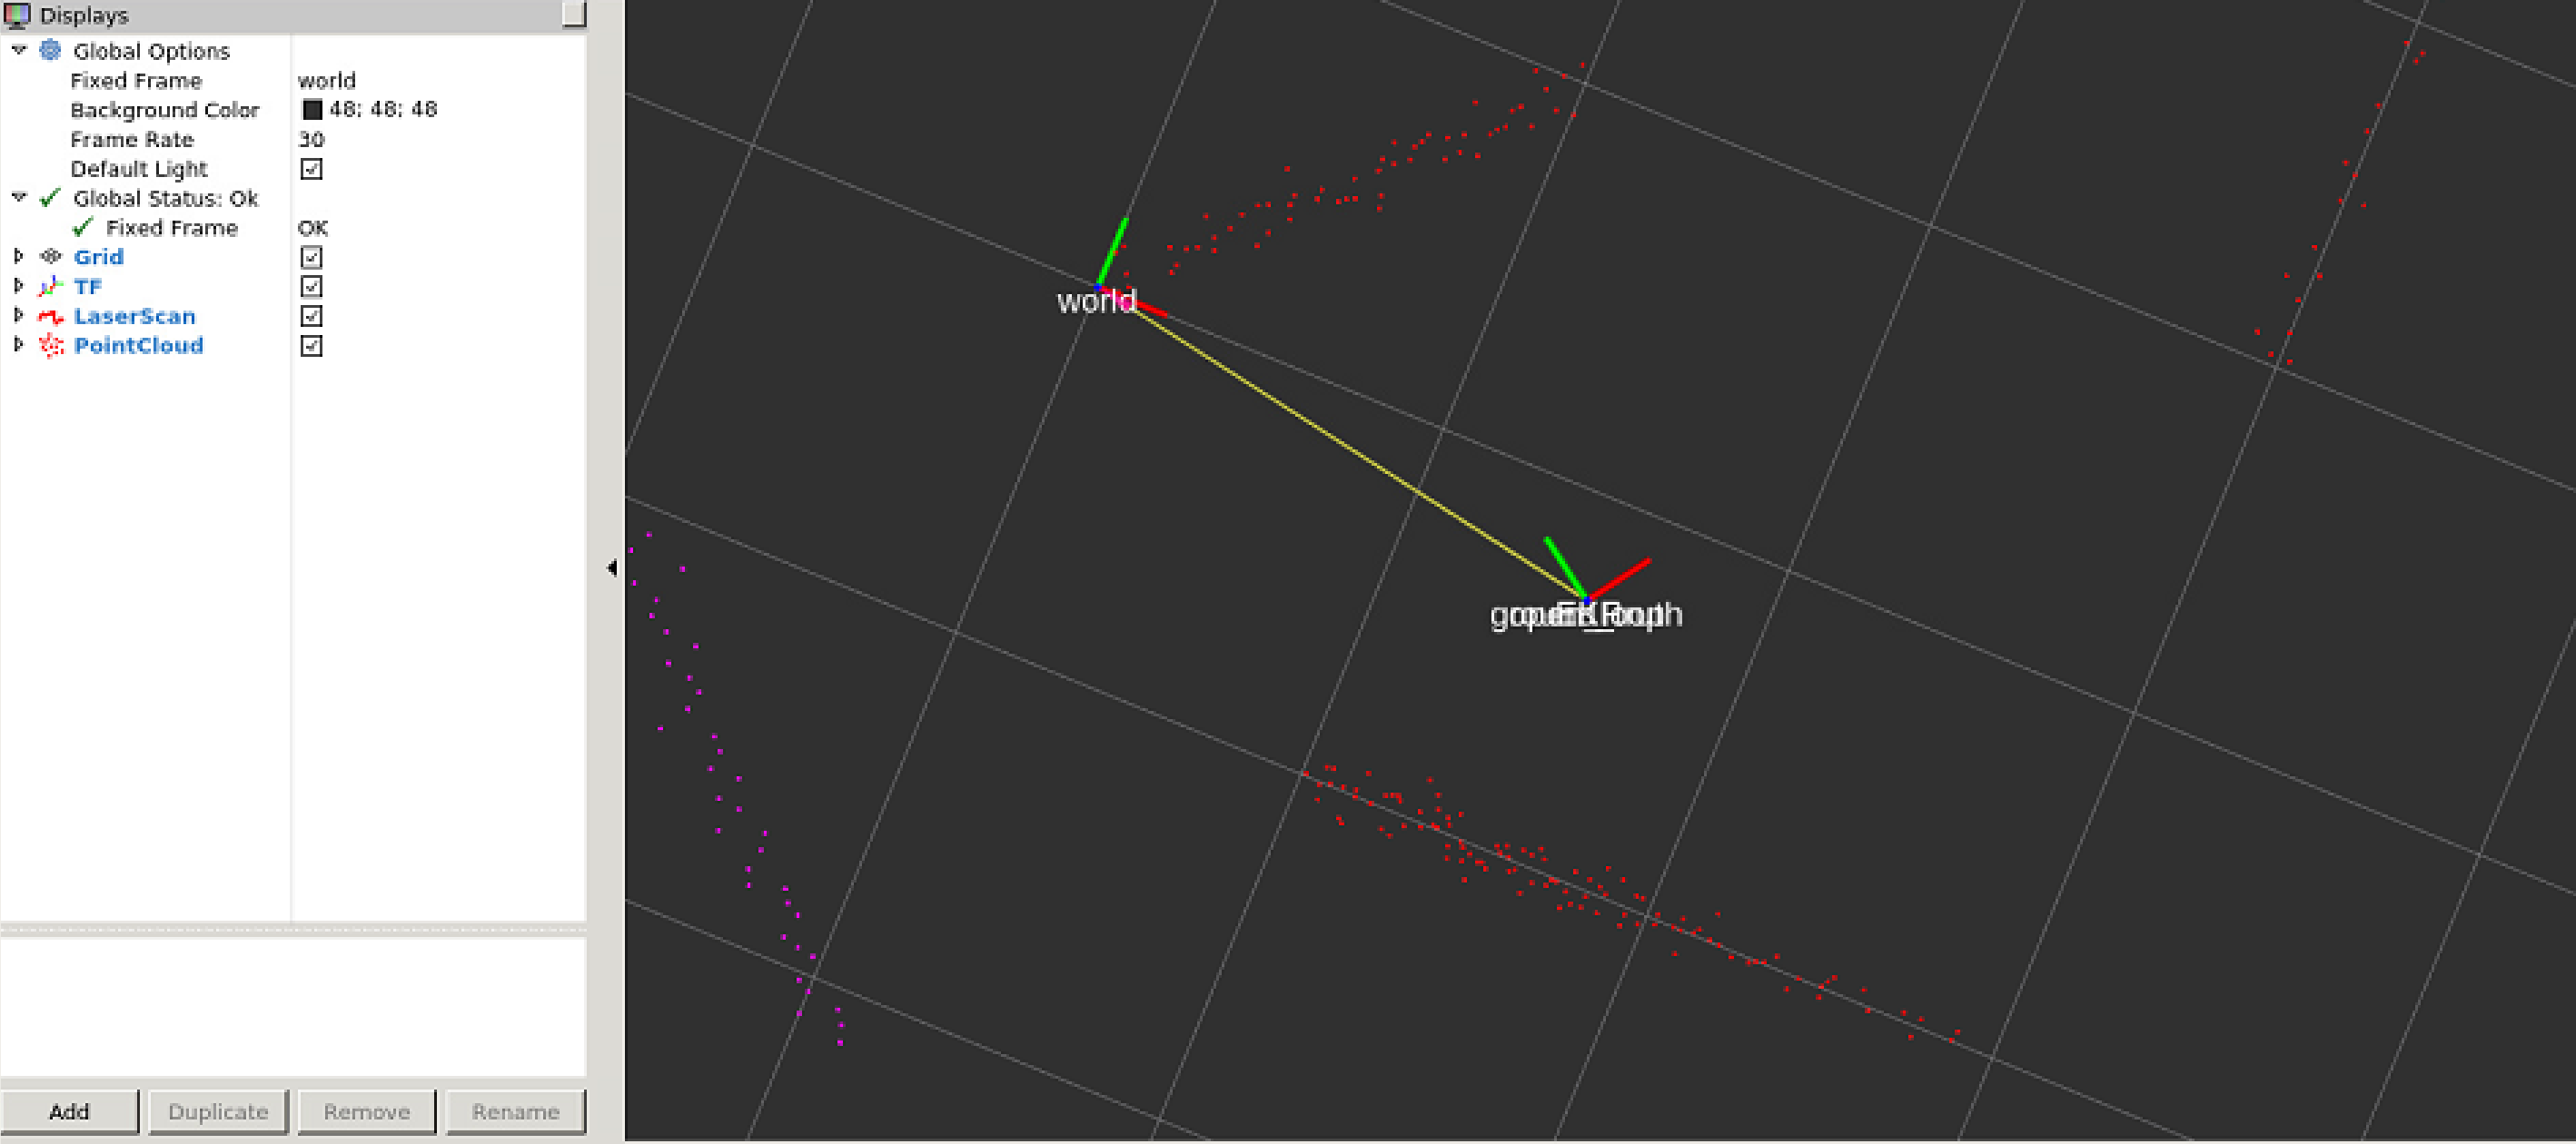
\includegraphics[width=0.65\textwidth]{P1_Screenshots/2move.PNG}
    \caption*{(2) The TurtleBot has moved far from the initial state}
    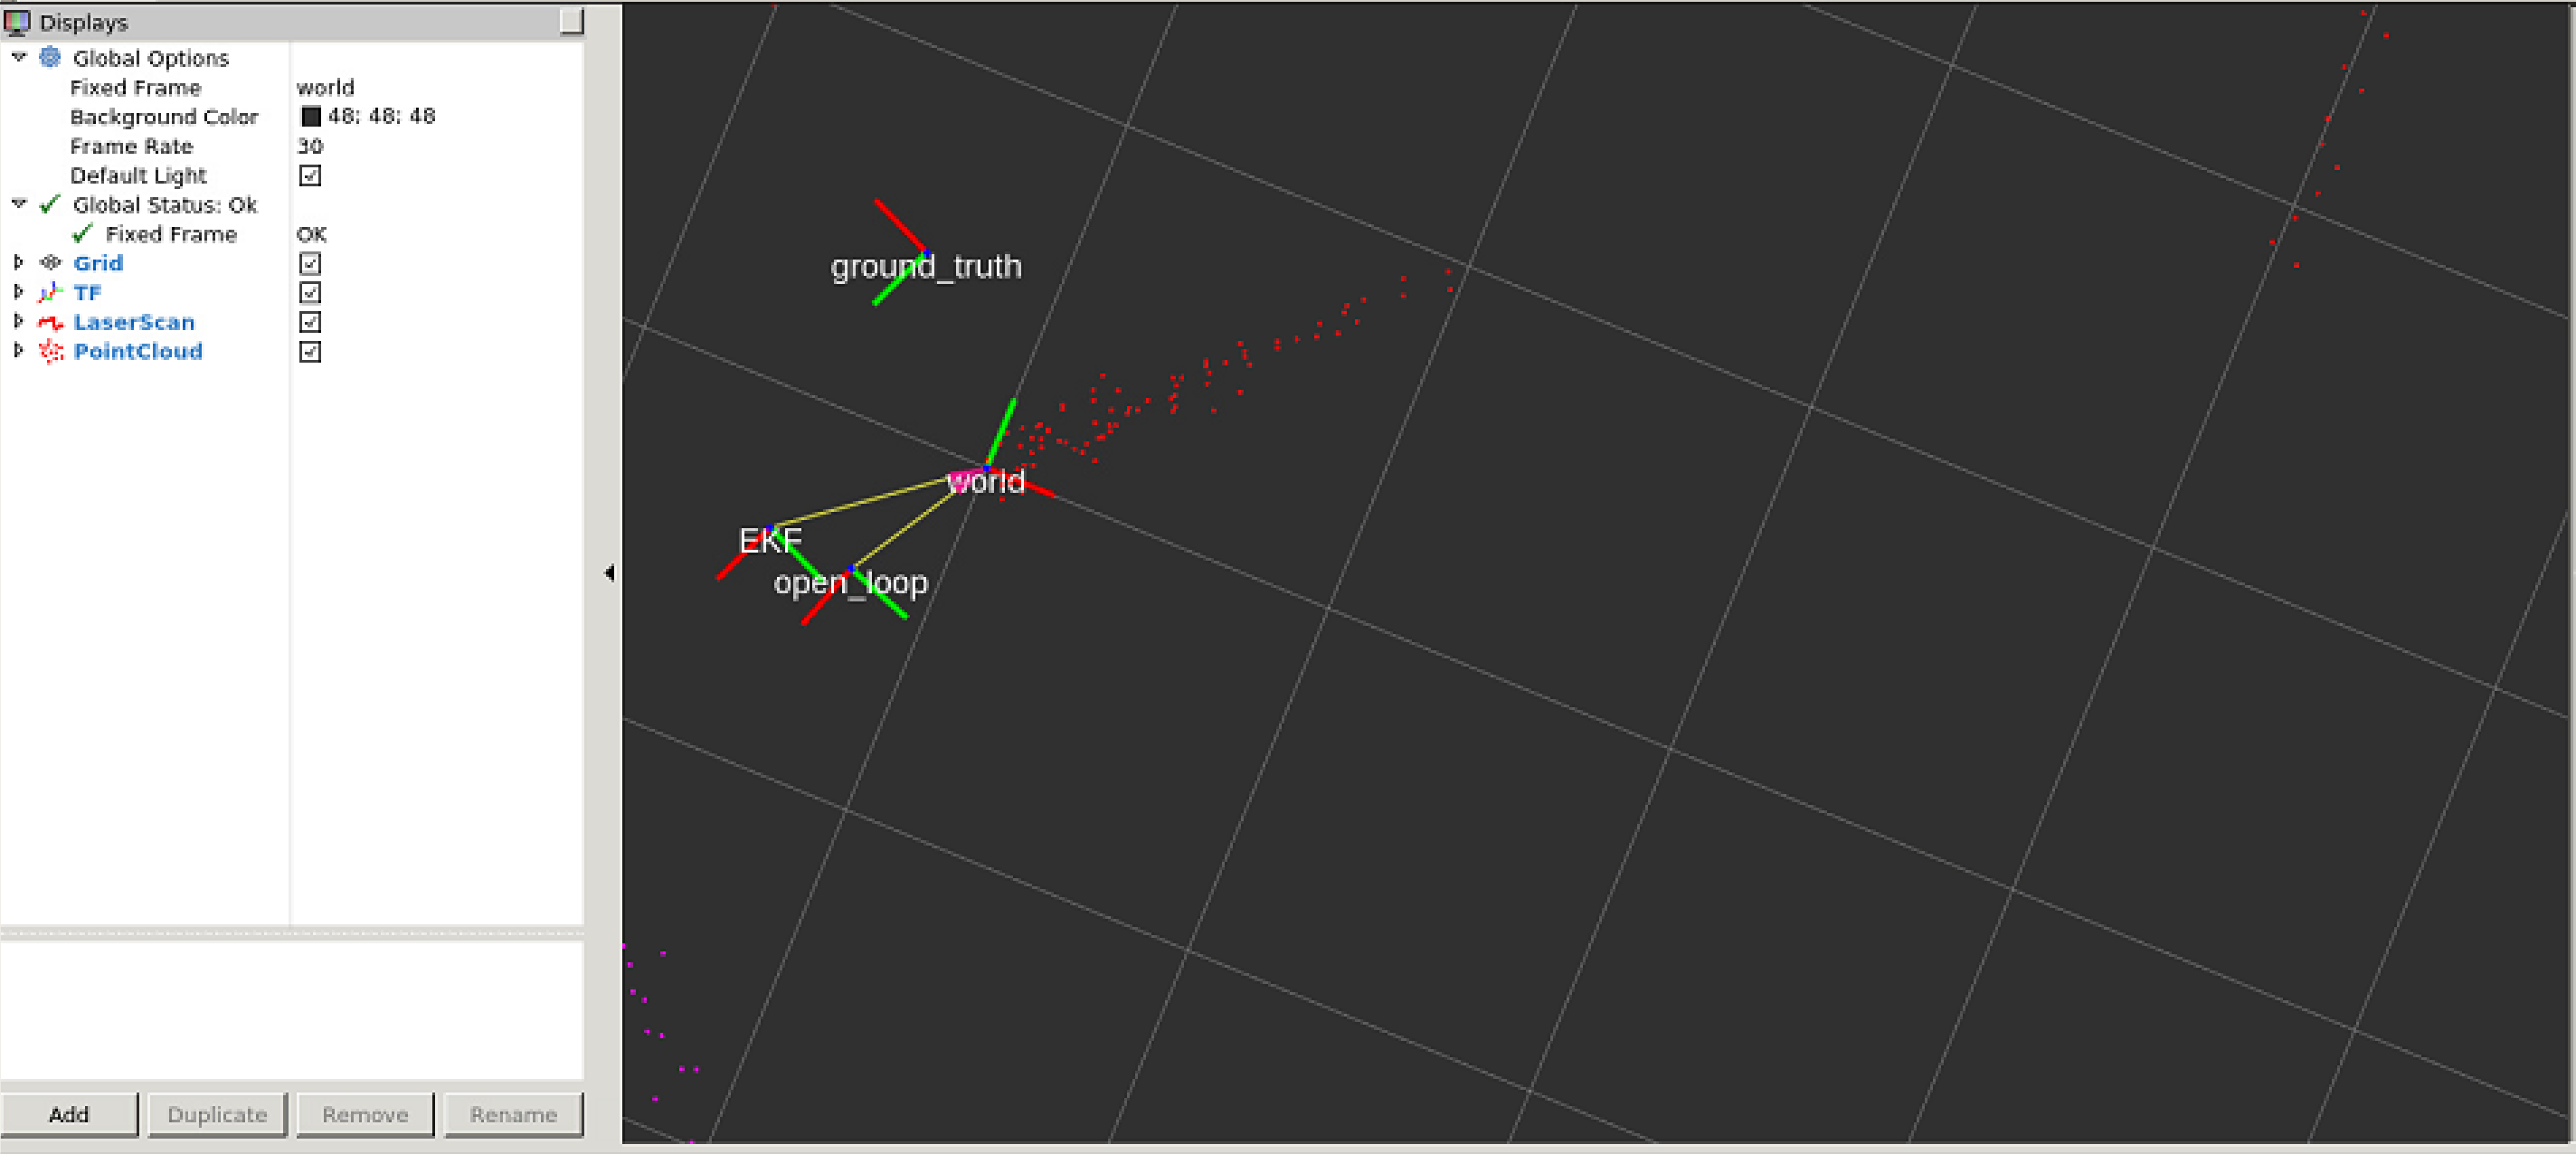
\includegraphics[width=0.65\textwidth]{P1_Screenshots/3diverge.PNG}
    \caption*{(3) The state estimates diverge}
    \end{center}
\end{figure}

\end{enumerate}

\newpage

\section*{Problem 2: EKF SLAM}
\begin{enumerate}[label=(\roman*)]
\item Implemented the computation of $g$, $G_x$, and $G_u$ in \codeword{transition_model()} in the \codeword{EkfSlam} class in \codeword{ekf.py}.
\item Reimplemented \codeword{measurement_model()}, \codeword{compute_innovations()}, and \\ \codeword{compute_predicted_measurements()} in the \codeword{EkfSlam} class. Below is \codeword{ekf_slam.png}.

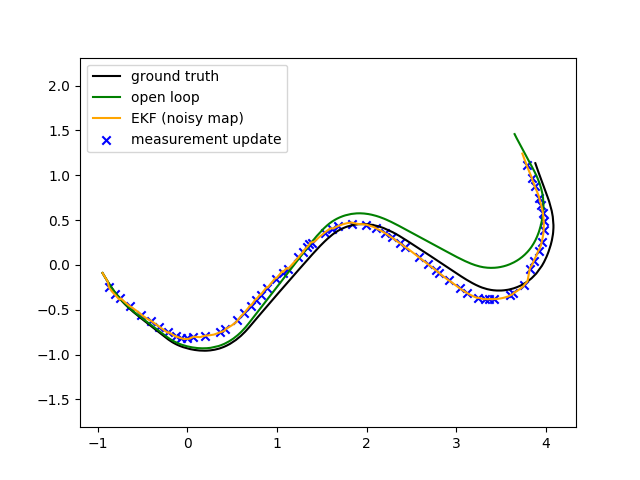
\includegraphics[width=\textwidth]{ekf_slam.png}

\item Copied the appropriate files to Genbu, launched \codeword{turtlebot3_arena.launch} and \\ \codeword{turtlebot3_teleop_key.launch}, and ran \codeword{map_fixing.py}. The EKF and ground truth diverge with fast rotations, changes in direction, or collisions with the walls. Screenshots are on the next page.

\begin{figure}[H]
    \begin{center}
    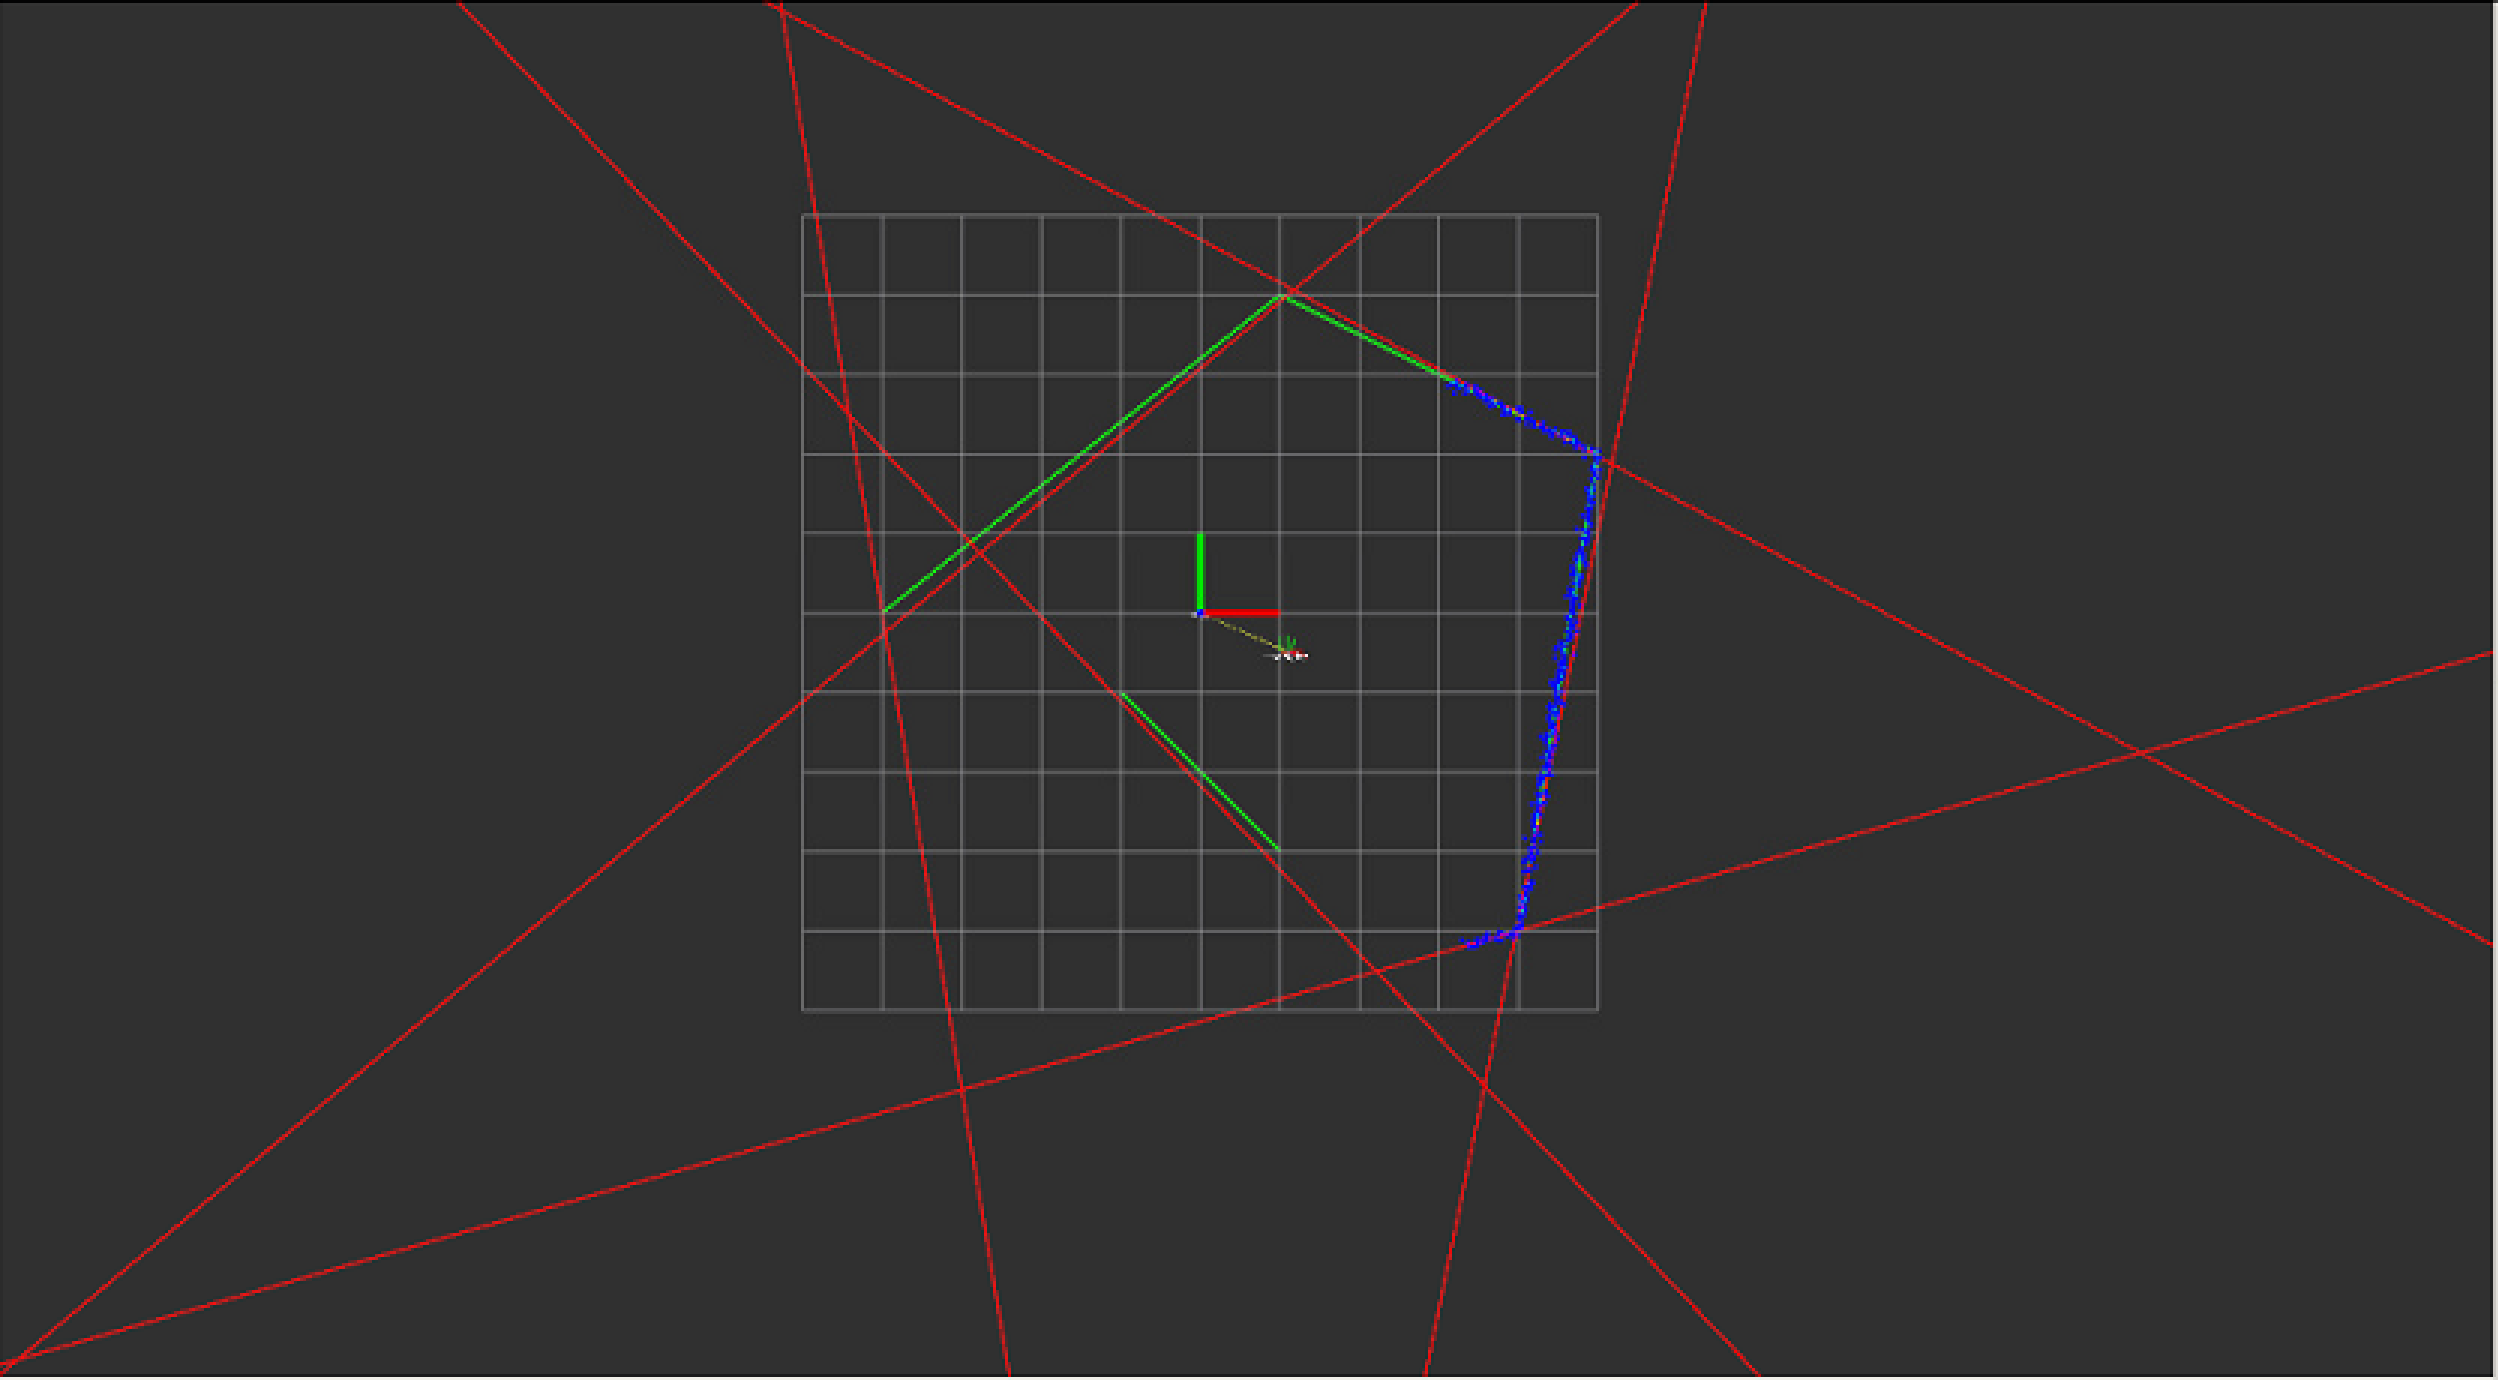
\includegraphics[width=0.65\textwidth]{P2_Screenshots/1initial.PNG}
    \caption*{(1) The initial state}
    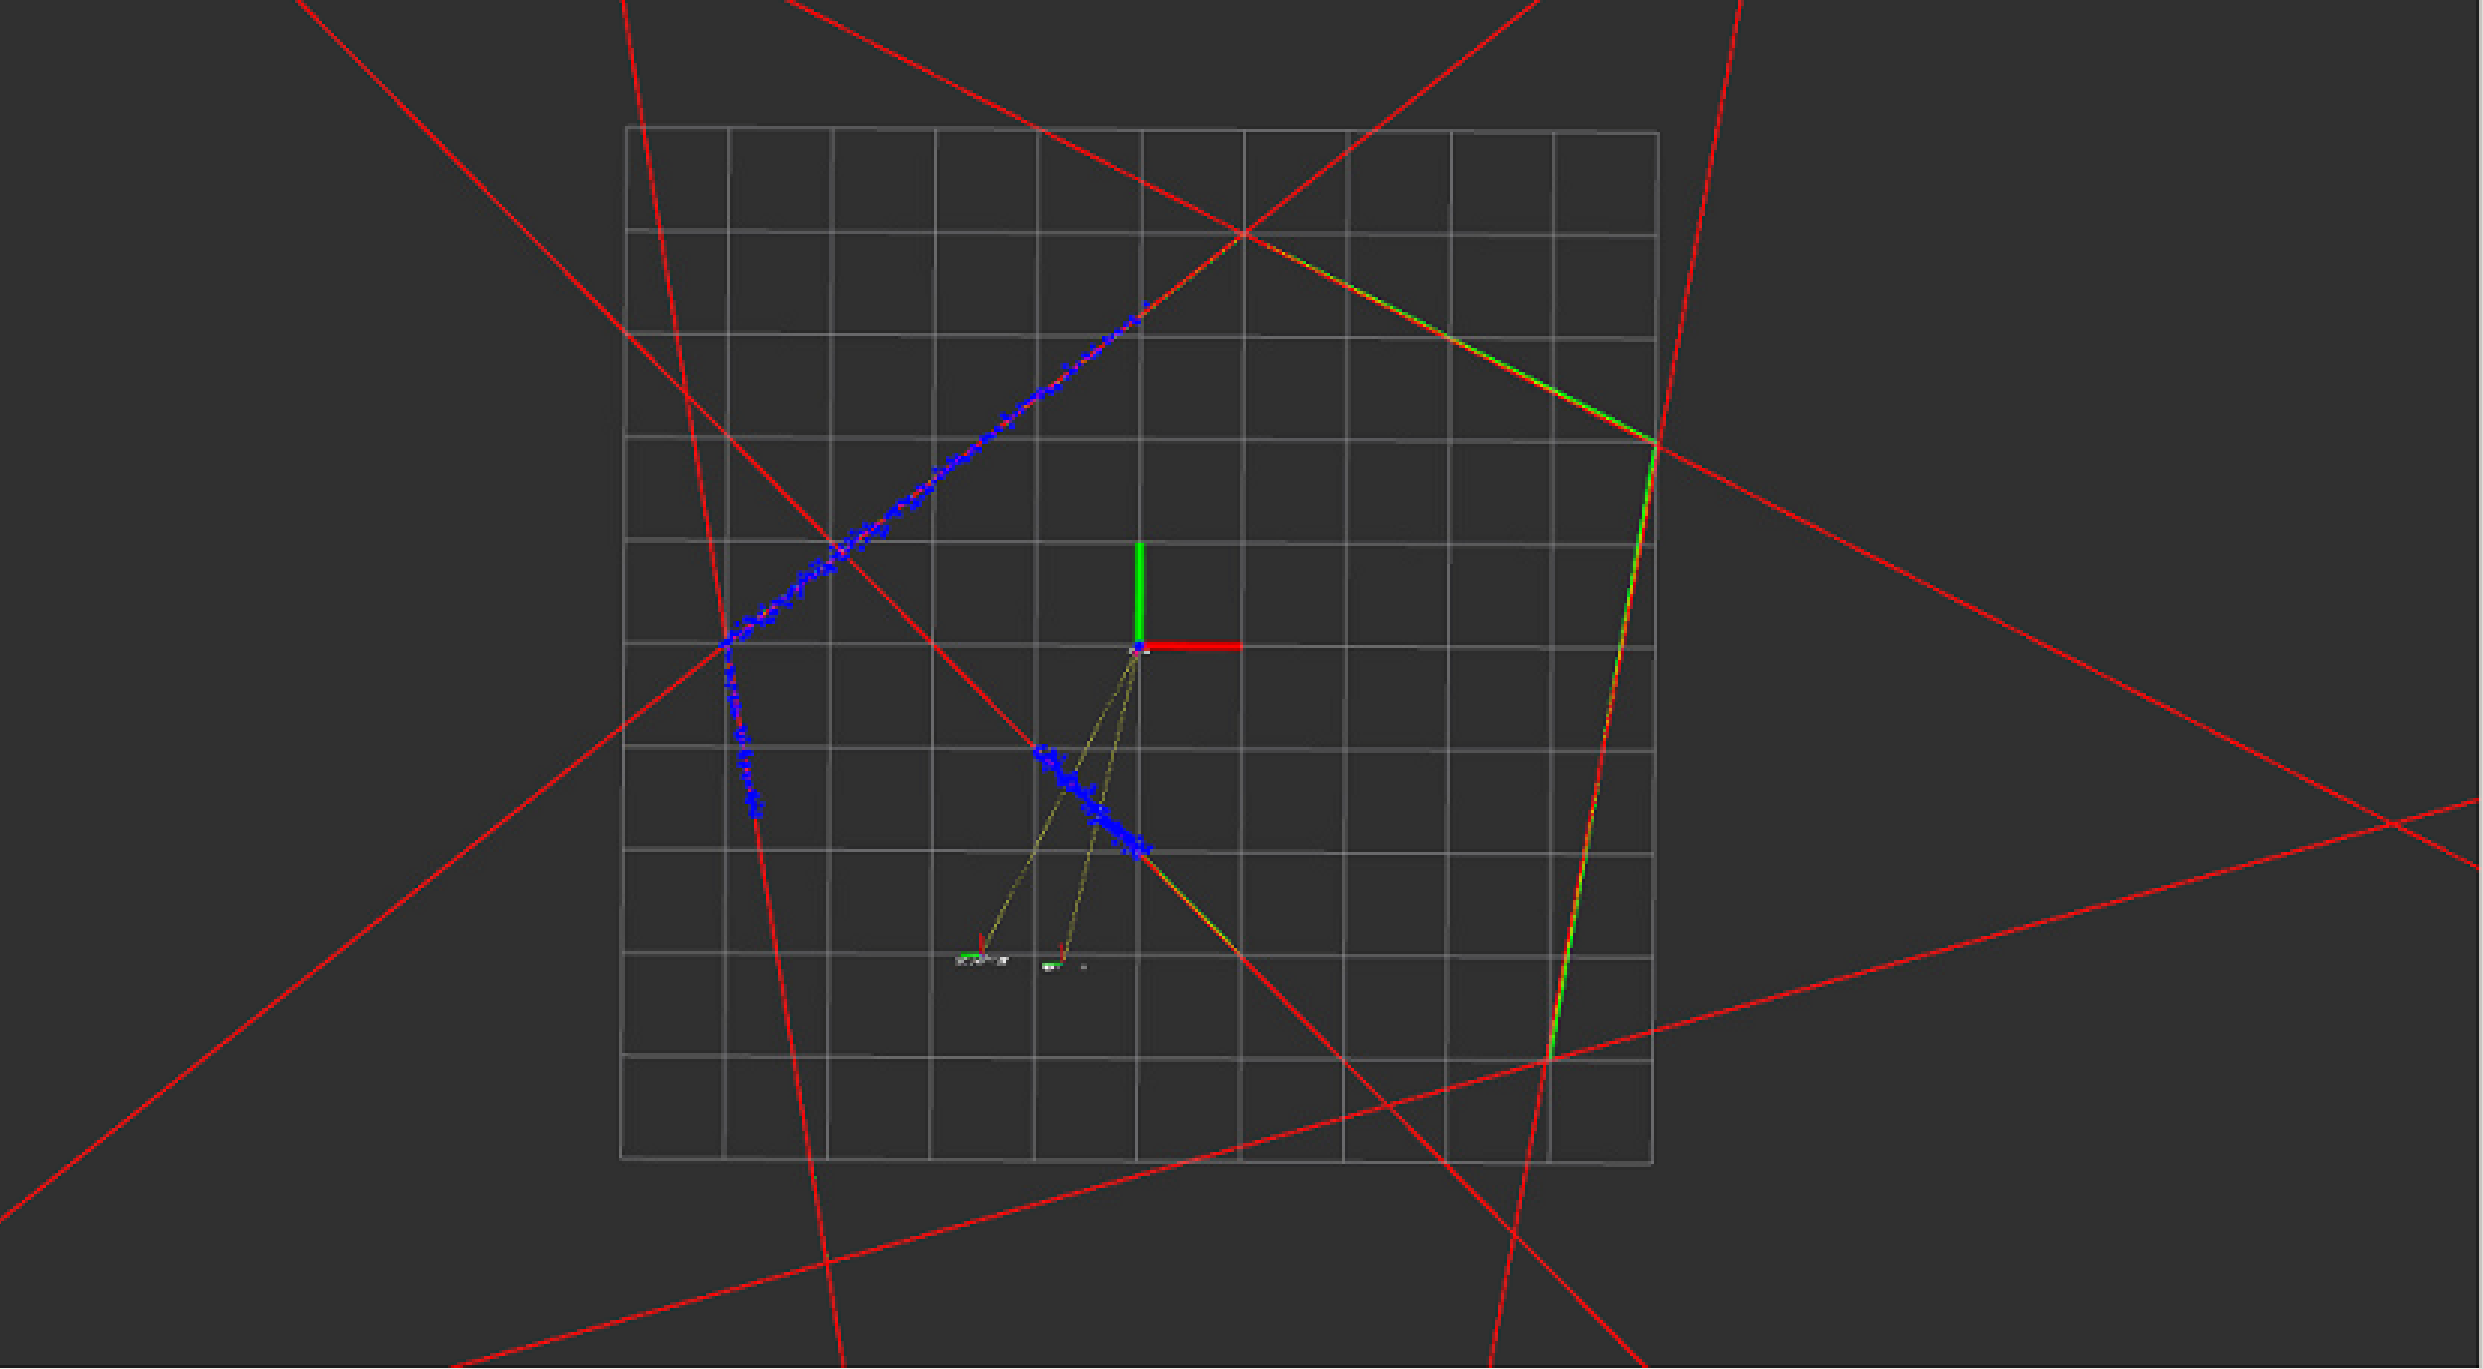
\includegraphics[width=0.65\textwidth]{P2_Screenshots/2moved.PNG}
    \caption*{(2) The TurtleBot has moved away from the initial state and the map estimate has changed}
    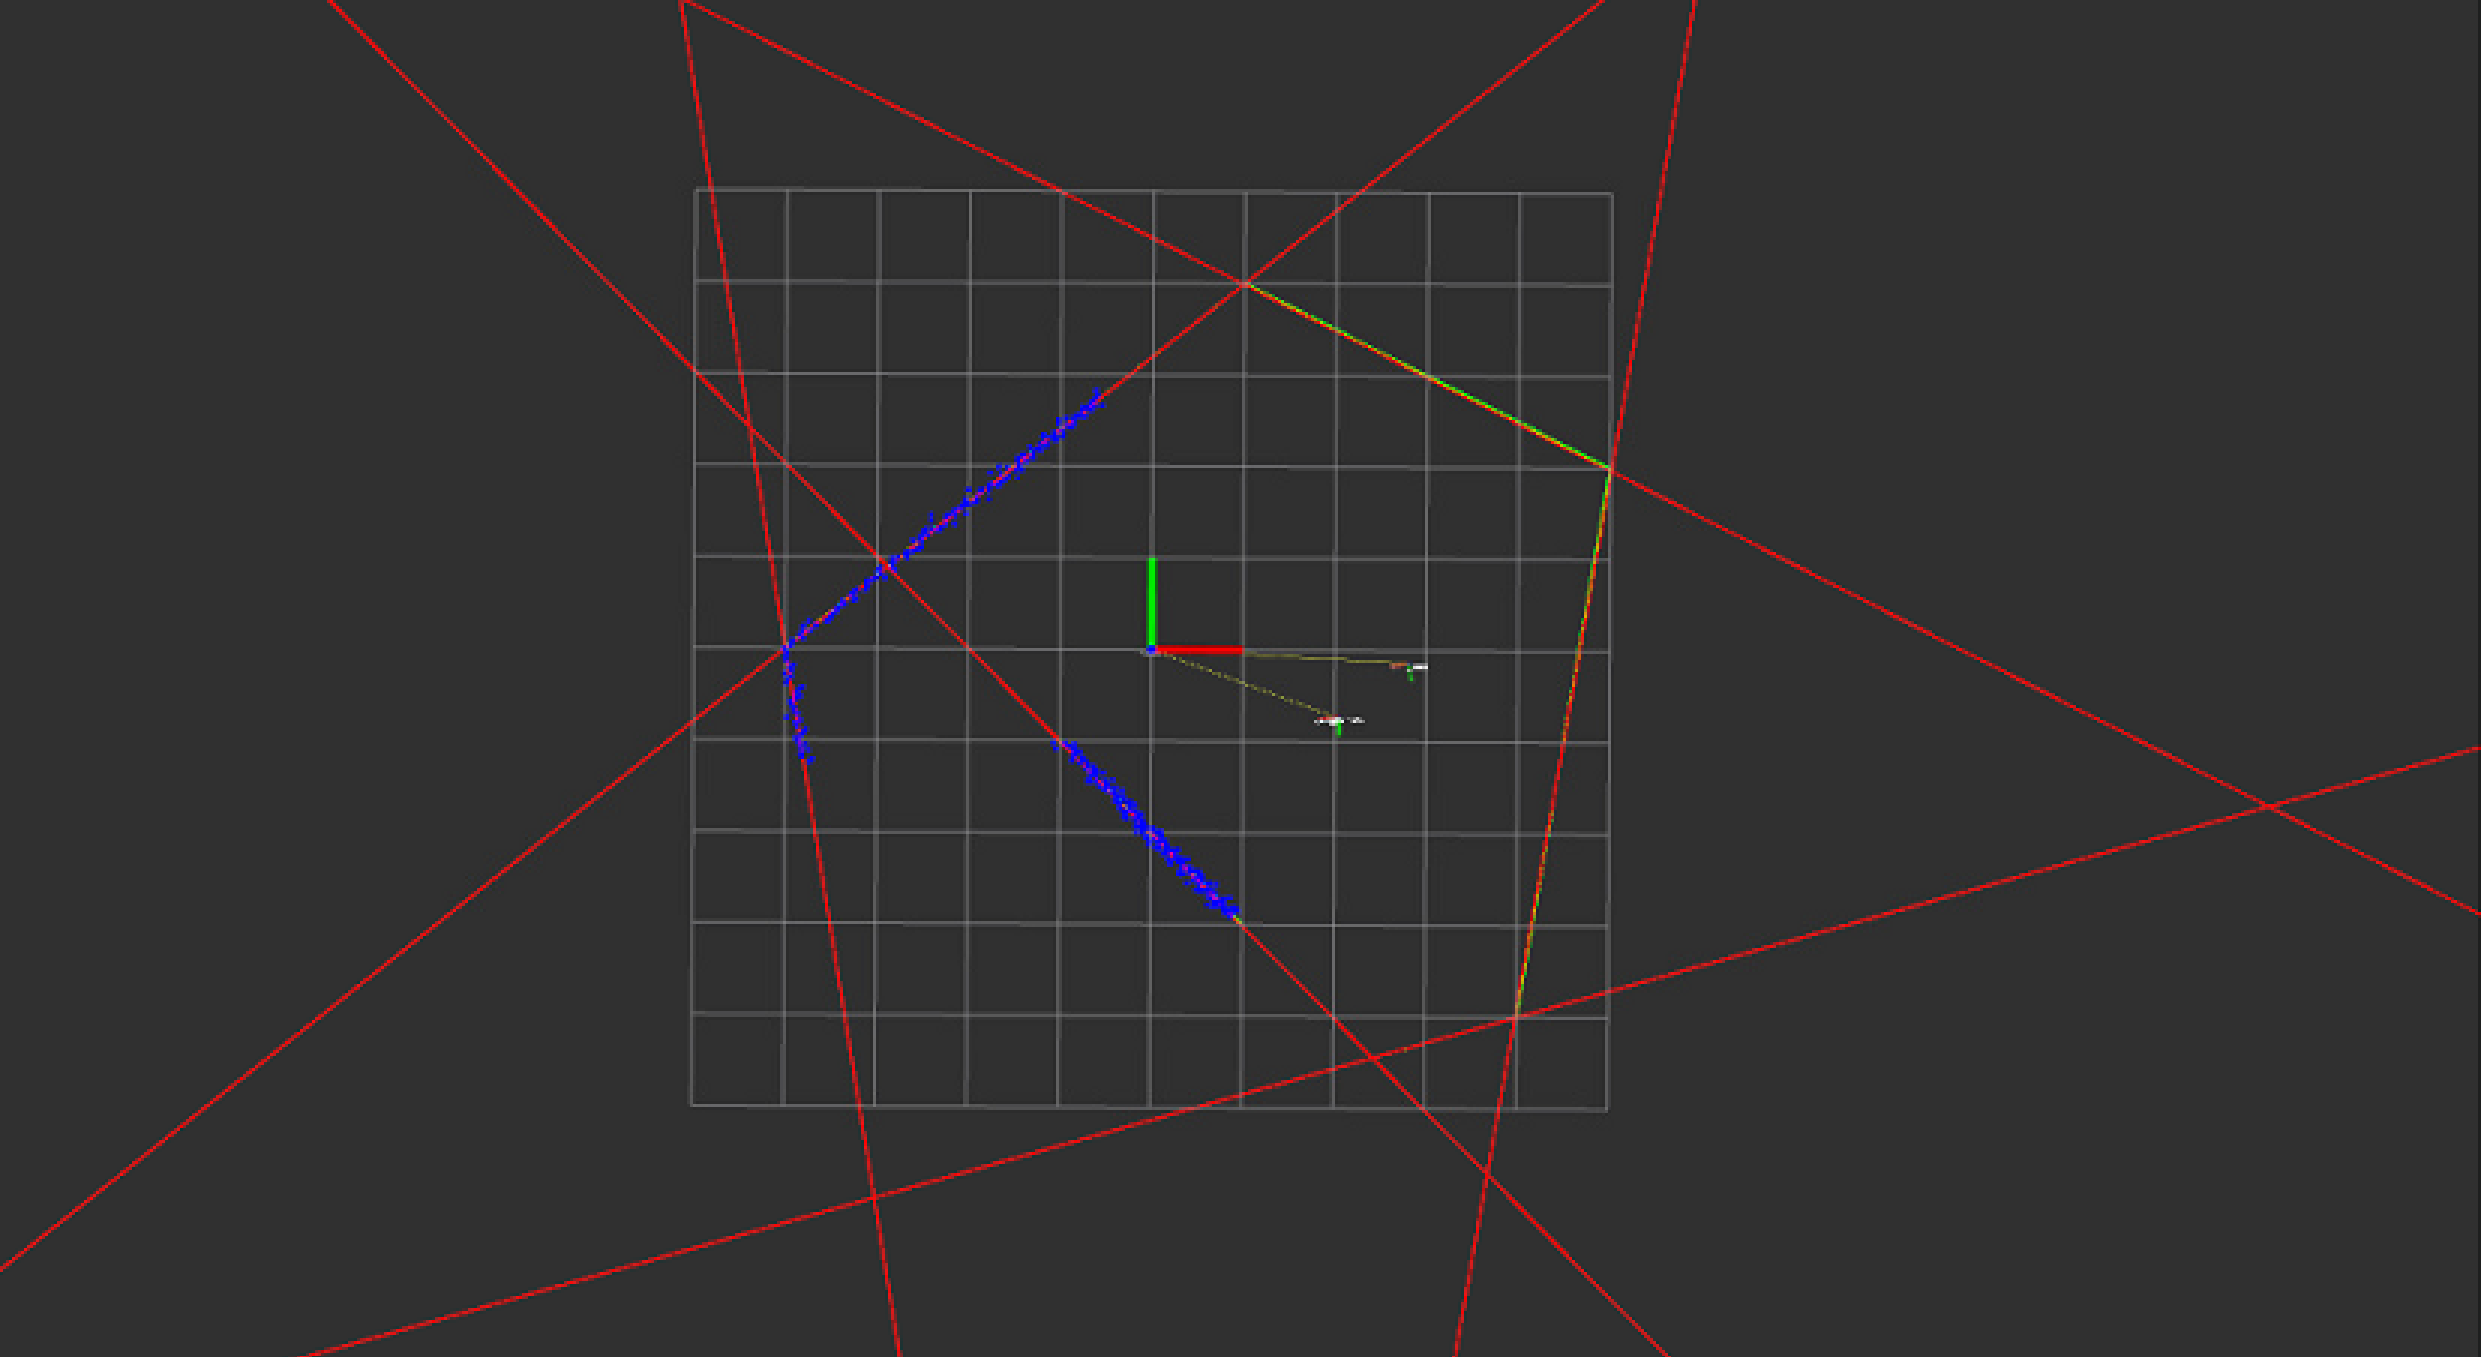
\includegraphics[width=0.65\textwidth]{P2_Screenshots/3converged.PNG}
    \caption*{(3) The map estimates have converged}
    \end{center}
\end{figure}

\end{enumerate}

\newpage

\section*{Extra Credit: Monte Carlo Localization}
\begin{enumerate}[label=(\roman*)]
\item Implemented the transition update step of MCL in \codeword{transition_model()} in the \codeword{ParticleFilter} class and \codeword{transition_update()} in the \codeword{MonteCarloLocalization} class in \codeword{particle_filter.py}.
\item Implemented the measurement update stepin \codeword{measurement_update()}, \codeword{measurement_model()}, \codeword{compute_innovations()}, and \codeword{compute_predicted_measurements()} in the \\ \codeword{MonteCarloLocalization} class in \codeword{particle_filter.py}.

\item Implemented \codeword{resample()} in the \codeword{ParticleFilter} class in \codeword{particle_filter.py}. Below is \codeword{mc_localization.png}.

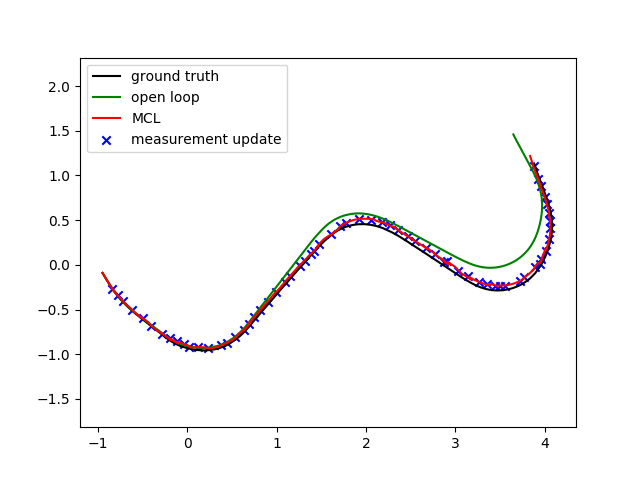
\includegraphics[width=\textwidth]{mc_localization.png}

\item Copied the appropriate files to Genbu, launched \codeword{turtlebot3_maze.launch} and \\ \codeword{turtlebot3_teleop_key.launch}, and ran \codeword{localization.py} with Monte Carlo enabled and 1000 particles. Similar to the EKF, with fast rotations or changes in direction, the MCL diverges but eventually is able to "correct" for the error. With more particles, the MCL is more tolerant to fast rotations and changes in direction. Screenshots are on the next page.

\begin{figure}[H]
    \begin{center}
    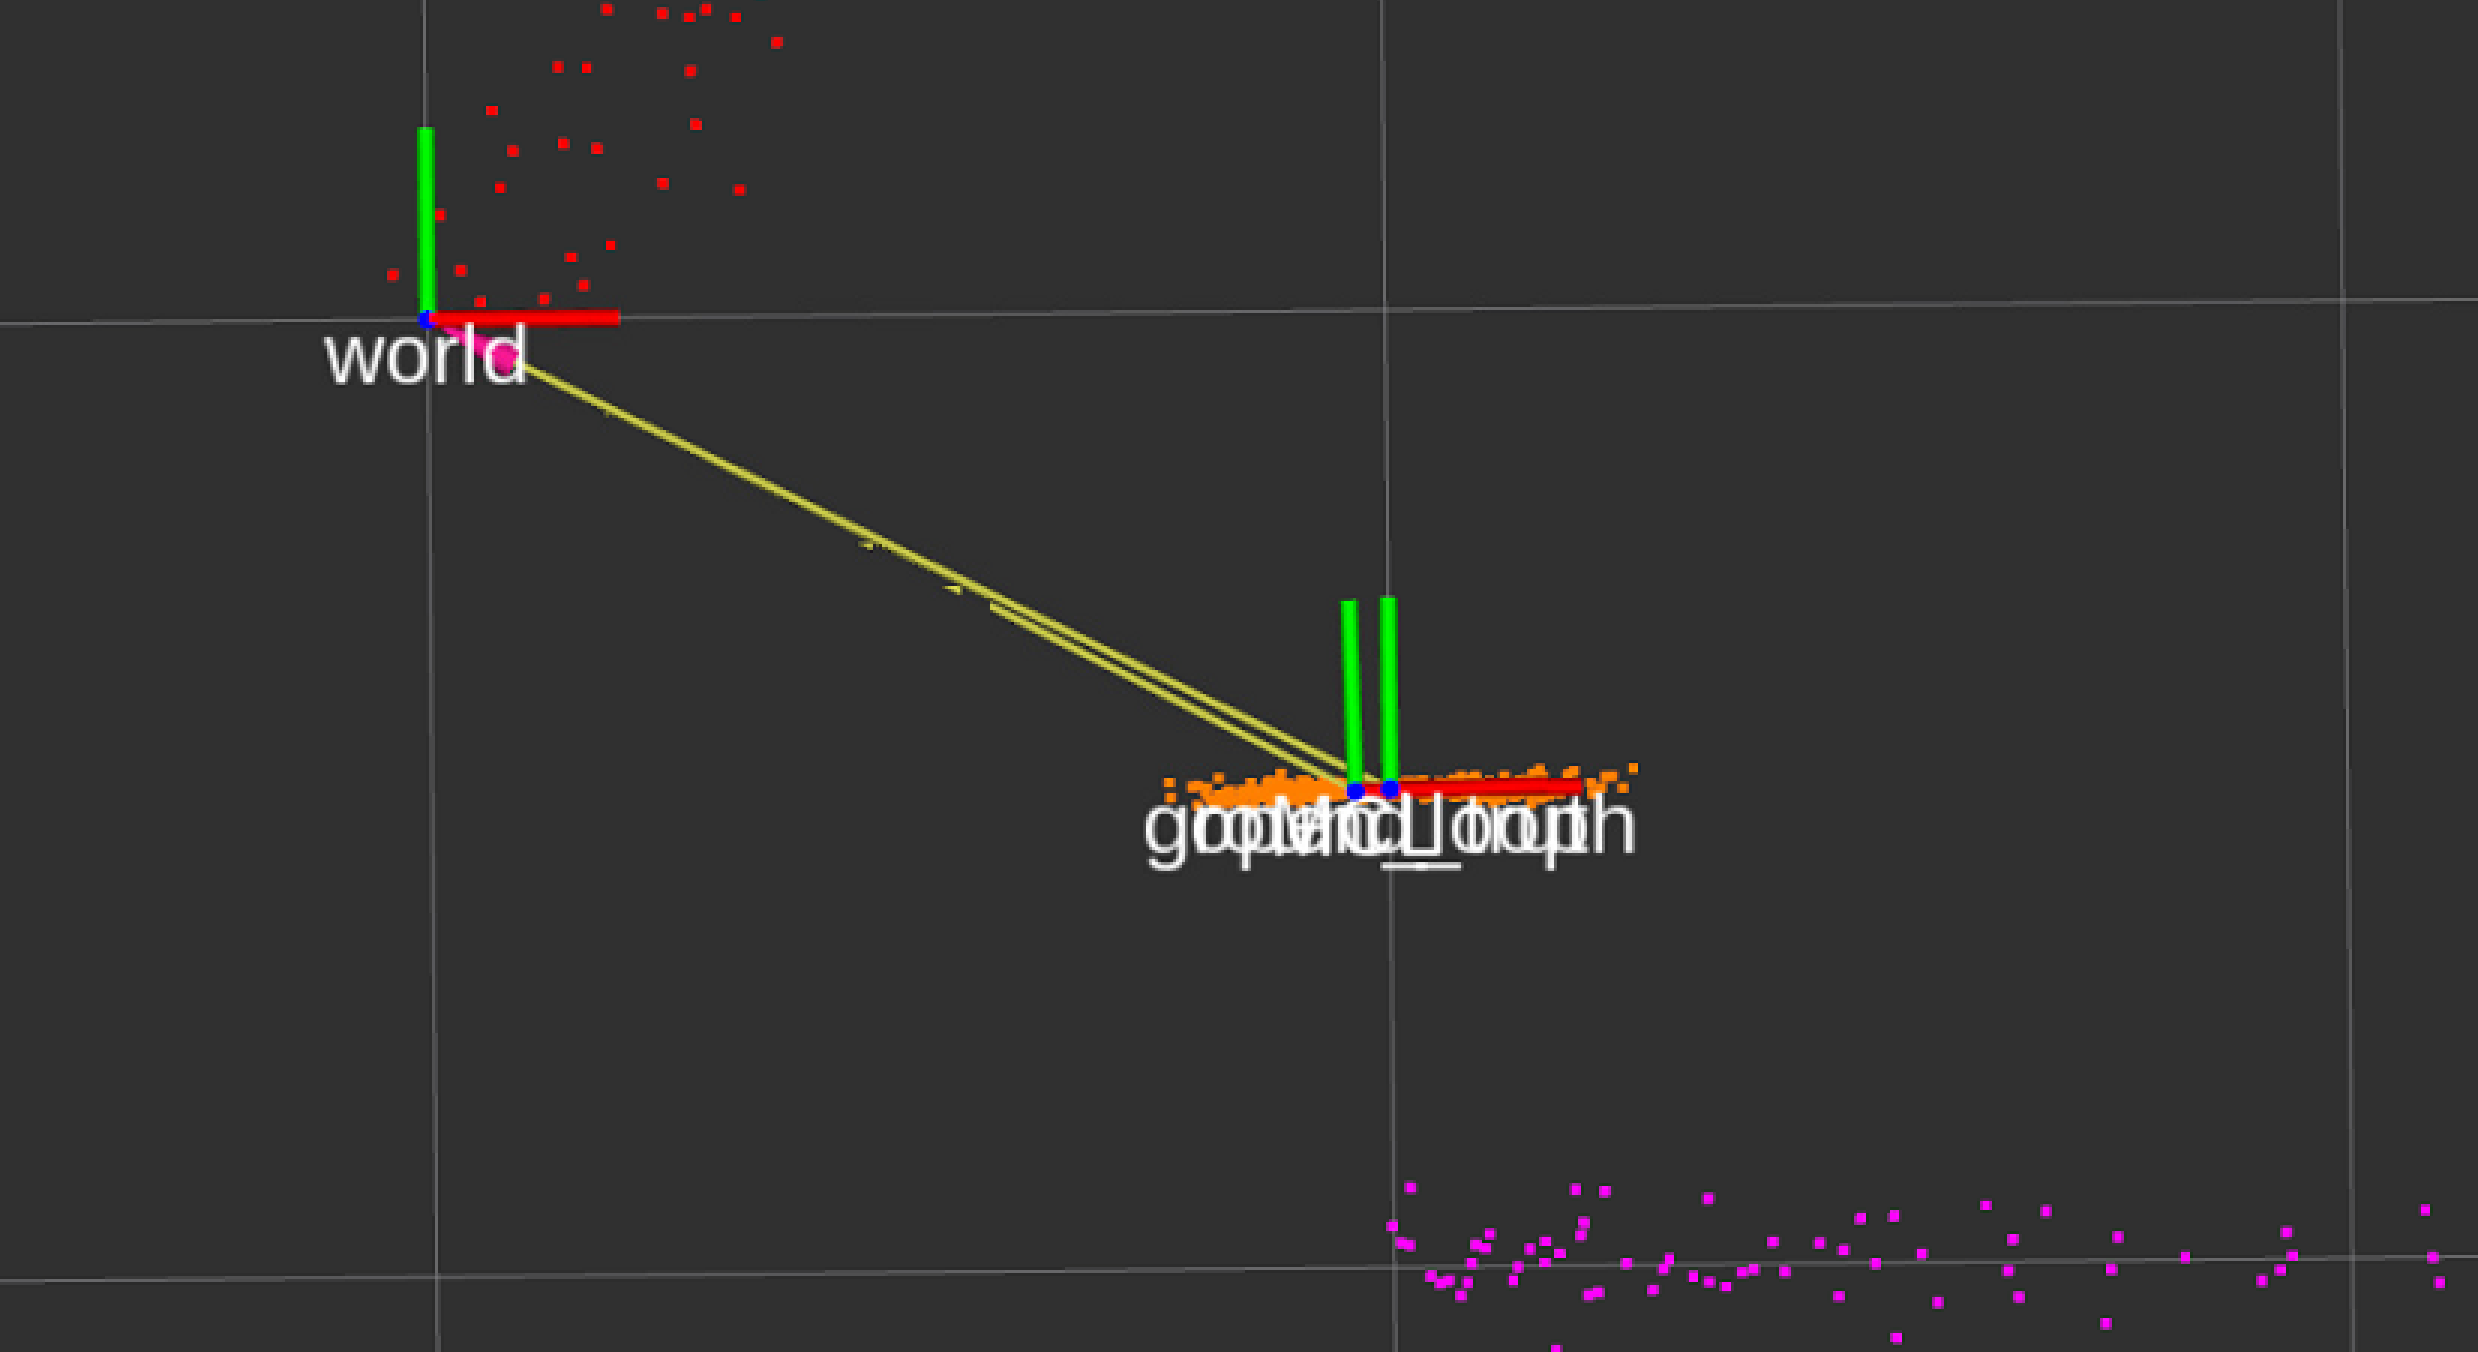
\includegraphics[width=0.65\textwidth]{P3_Screenshots/1initial.PNG}
    \caption*{(1) The initial state}
    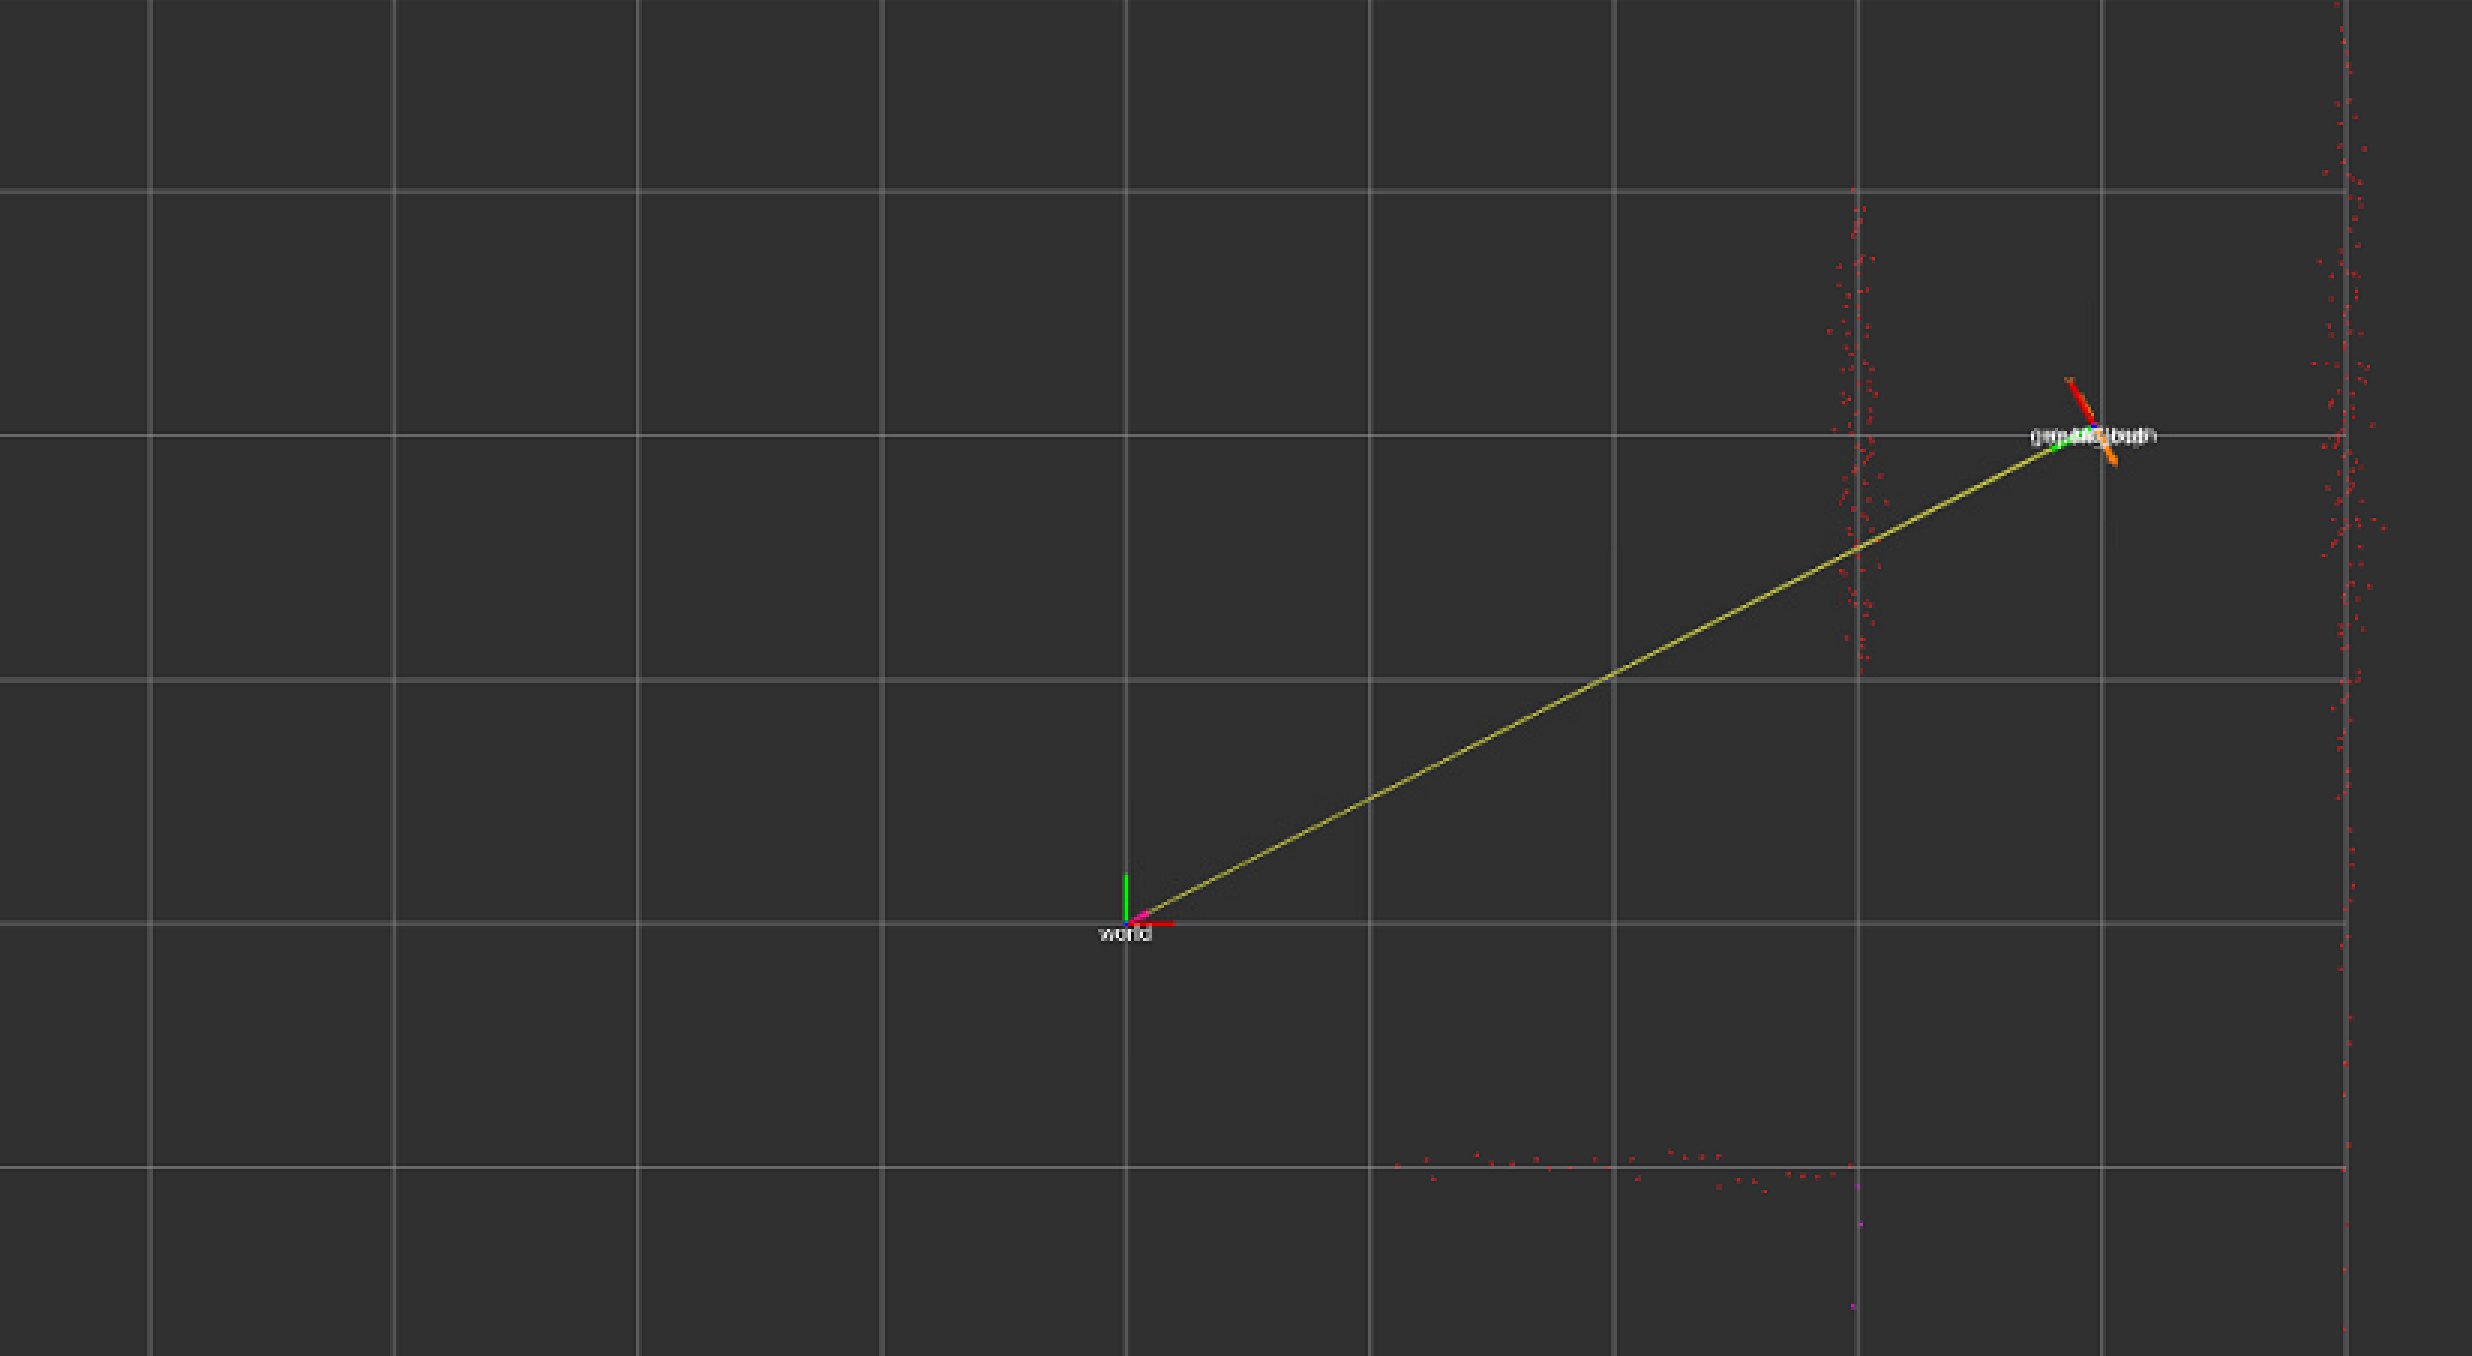
\includegraphics[width=0.65\textwidth]{P3_Screenshots/2moved.PNG}
    \caption*{(2) The TurtleBot has moved far from the initial state}
    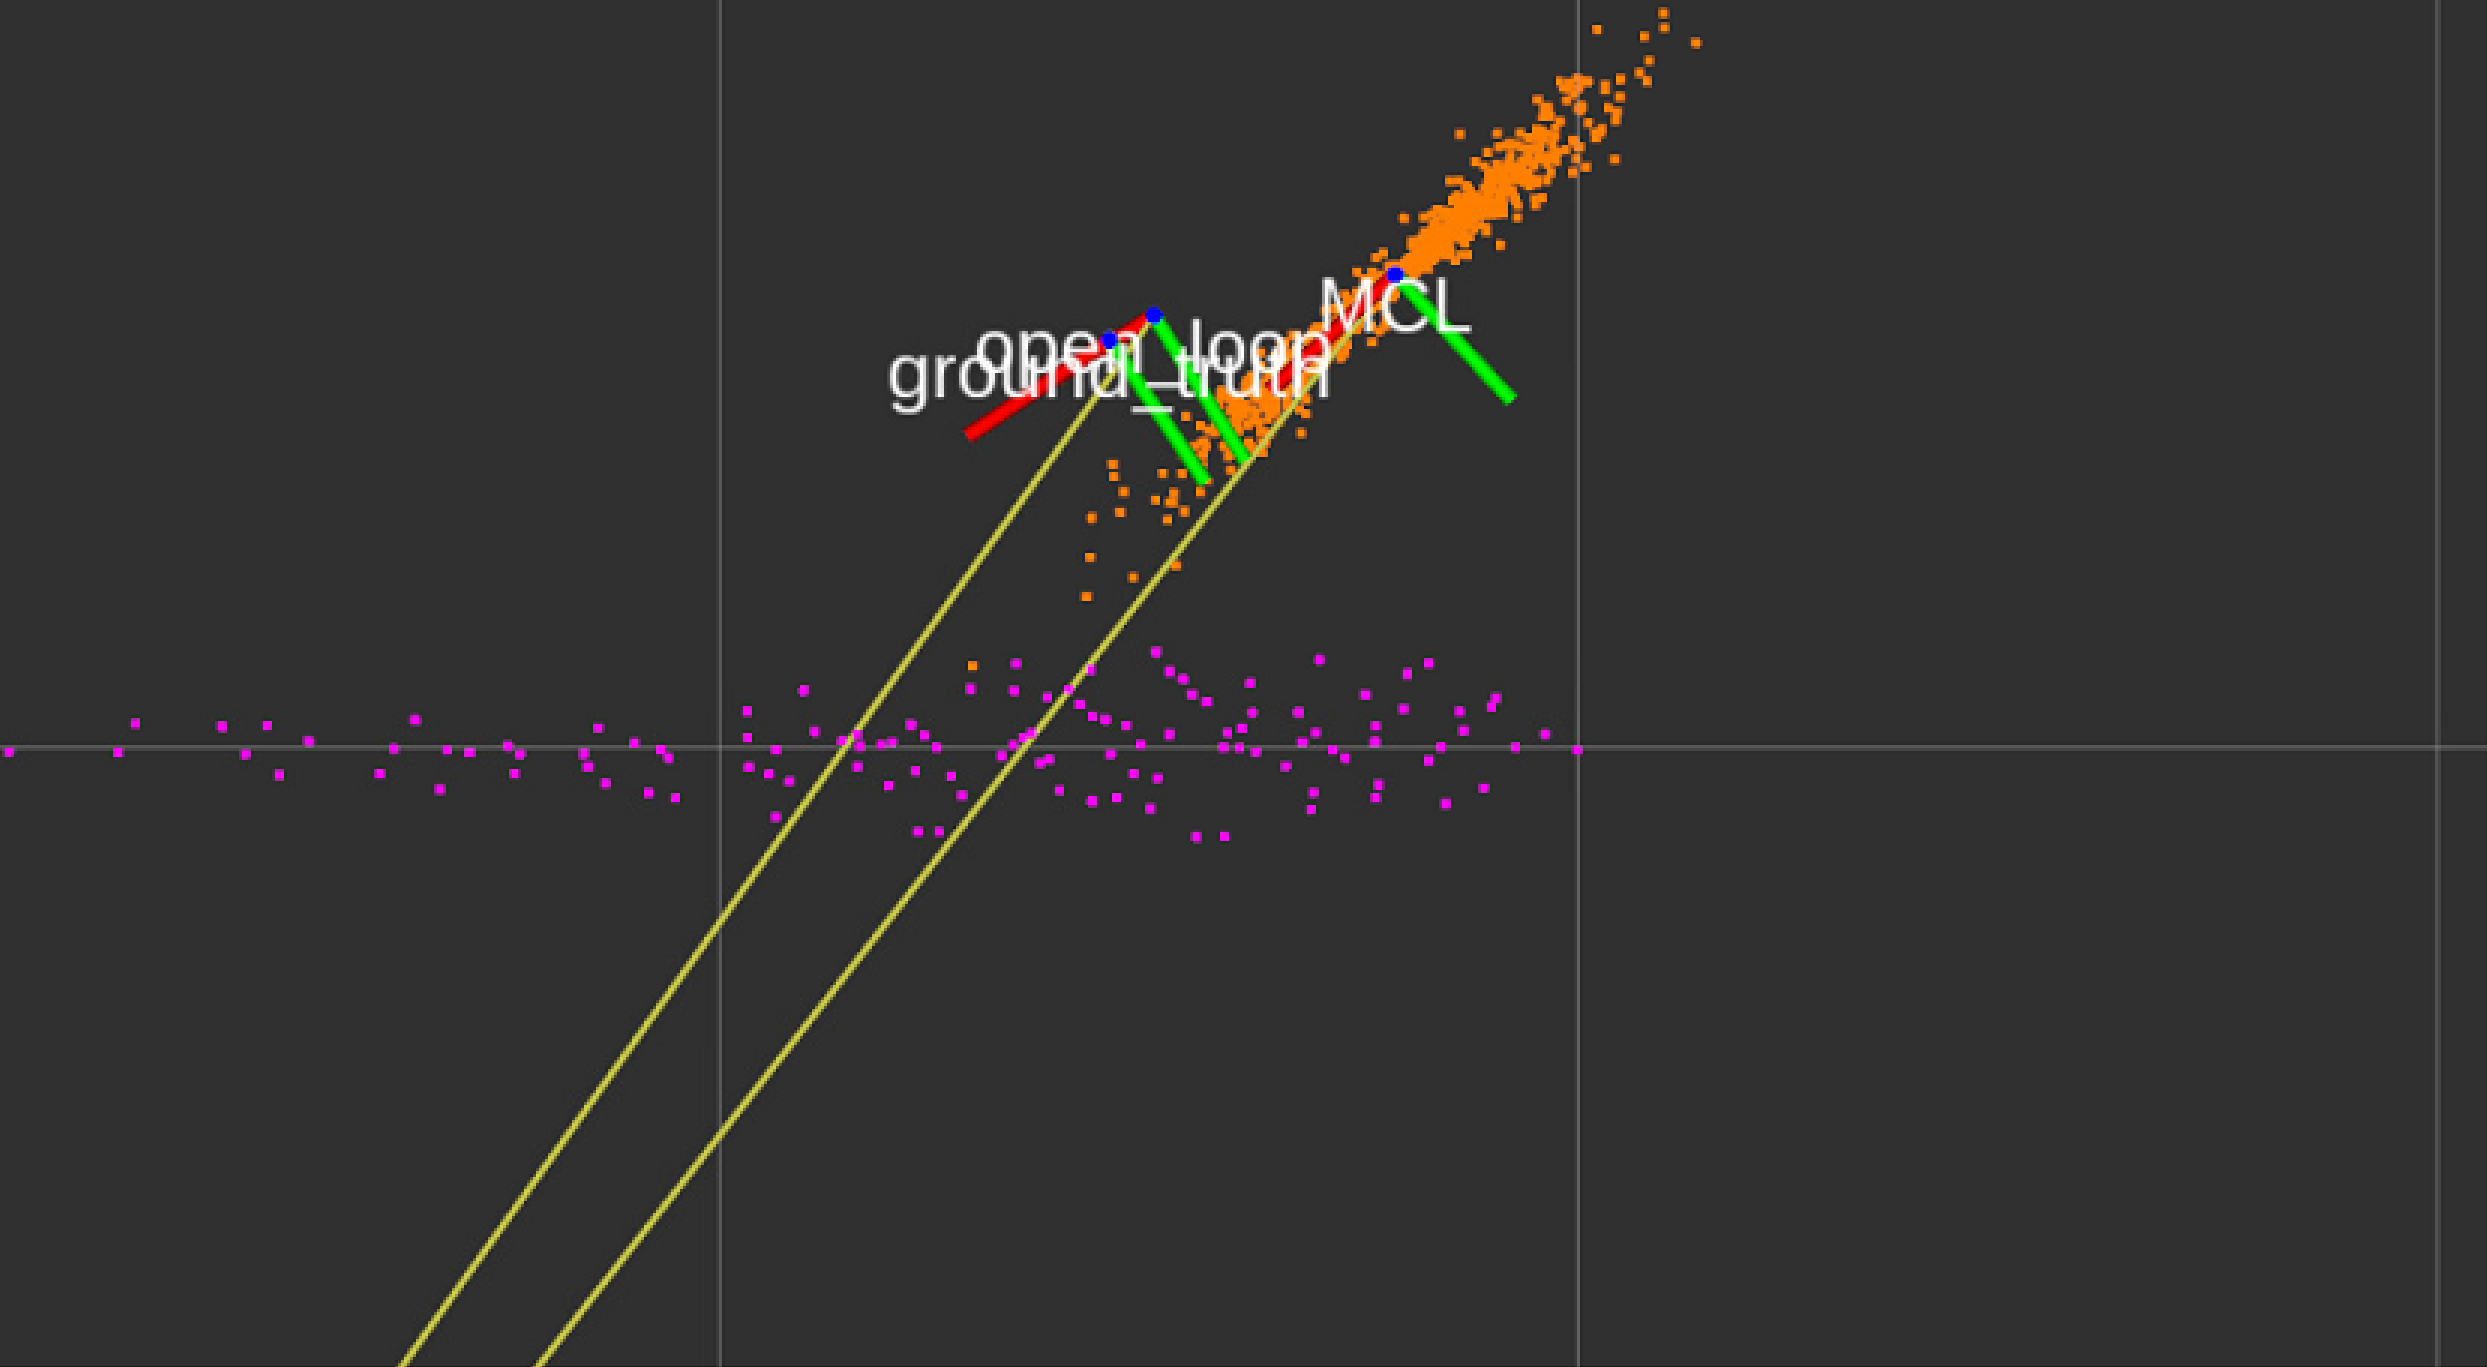
\includegraphics[width=0.65\textwidth]{P3_Screenshots/3diverged.PNG}
    \caption*{(3) The state estimates have diverged}
    \end{center}
\end{figure}

\newpage

\item Vectorized all functions. The code is below.
\begin{minted}{python}
def resample(self, xs, ws):
    r = np.random.rand() / self.M
    ws_cumsum = np.cumsum(ws)
    ws_total = ws_cumsum[-1] # last element in ws_cumsum is the overall total
    m = np.linspace(0, self.M, self.M, False) # 0, 1, 2, ... M-1
    u = ws_total * (r + m/self.M)
    particle_idxs = np.searchsorted(ws_cumsum, u)
    self.xs = xs[particle_idxs]
    self.ws = ws[particle_idxs]
    
def transition_model(self, us, dt):
    g = np.zeros((self.M, 3))
    theta = self.xs[...,2]
    x = self.xs[...,0]
    y = self.xs[...,1]
    V = us[...,0]
    w = us[...,1]
    s_w = w

    sin_t = np.sin(theta) + np.sin(theta + w*dt)
    cos_t = np.cos(theta) + np.cos(theta + w*dt)
    g1 = np.stack([x + V*0.5*cos_t*dt, y + V*0.5*sin_t*dt, theta + w*dt], -1)

    inv_w = 1.0 / np.maximum(np.abs(w),EPSILON_OMEGA)*np.sign(w)
    n_theta = theta + s_w * dt
    upper_sin = np.sin(n_theta)
    lower_sin = np.sin(theta)
    upper_cos = np.cos(n_theta)
    lower_cos = np.cos(theta)
    g2 = np.stack([x + V*inv_w*(upper_sin - lower_sin), 
                   y + V*inv_w*(-upper_cos + lower_cos), theta + w*dt], -1)

    g = np.where(np.abs(w[:,None])<EPSILON_OMEGA, g1, g2)
    return g
\end{minted}
\newpage
\begin{minted}{python}
        
def compute_innovations(self, z_raw, Q_raw):
    J = self.map_lines.shape[1]
    I = z_raw.shape[1]

    hs = self.compute_predicted_measurements().transpose(0, 2, 1) # (M, J, 2)

    z_matrix = z_raw.T[None, None, :, :] # (1, 1, I, 2)
    h_matrix = hs[:, :, None, :] # (M, J, 1, 2)
    
    # Vectorized angle_diff
    z_alpha = z_matrix[..., 0] % (2.*np.pi) # (M, J, I)
    h_alpha = h_matrix[..., 0] % (2.*np.pi)
    angle_diffs = z_alpha - h_alpha 
    idxs = np.pi < angle_diffs
    signs = 2 * (angle_diffs[idxs] < 0) - 1
    angle_diffs[idxs] += signs * 2. * np.pi
    innovations_alpha = angle_diffs

    innovations_r = z_matrix[..., 1] - h_matrix[..., 1]
    innovations = np.stack((innovations_alpha, innovations_r), axis=3)

    v = innovations[..., None] # (M, J, I, 2, 1)
    Q_inv = np.linalg.inv(Q_raw)[None, None, :, :, :] # (1, 1, I, 2, 2)
    
                                                        # (M, J, I, 1, 1)
    d_matrix = np.matmul(np.matmul(v.transpose(0, 1, 2, 4, 3), Q_inv), v) 
    d_matrix = d_matrix.reshape((self.M, J, I))  # (M, J, I)

    d_argmin = np.argmin(d_matrix, axis=1)[:, None, :, None] # (M, 1, I, 1)
    vs = np.take_along_axis(innovations, d_argmin, axis=1) # (M, 1, I, 2)
    vs = vs.reshape((self.M, I, 2)) # (M, I, 2)

    # Reshape [M x I x 2] array to [M x 2I]
    return vs.reshape((self.M,-1))  # [M x 2I]

\end{minted}
\newpage
\begin{minted}{python}
def compute_predicted_measurements(self):
    
    J = self.map_lines.shape[1]

    hs = self.map_lines.T # (J, 2)
    alpha, r = hs[:, 0], hs[:, 1]

    # Vectorized transform_line_to_scanner_frame
    x_cam, y_cam, th_cam = self.tf_base_to_camera
    x_base, y_base, th_base = self.xs.T

    tf_robot_to_world = np.array([[np.cos(th_base), -np.sin(th_base), x_base],
                                  [np.sin(th_base),  np.cos(th_base), y_base], 
                                  [              0,                0,      1]])
    
    x_cam_world, y_cam_world, th_cam_world =
            tf_robot_to_world.dot(np.array([x_cam, y_cam, 1]))


    alpha_cam = alpha[None, :] - th_base[:, None] - th_cam
    r_cam = (r[None, :] - x_cam_world[:, None]*np.cos(alpha)[None, :]
                        - y_cam_world[:, None]*np.sin(alpha)[None, :])
    
    # Vectorized normalize_line_parameters
    idxs = r_cam < 0
    alpha_cam[idxs] += np.pi
    r_cam[idxs] *= -1
    alpha_cam = (alpha_cam + np.pi) % (2*np.pi) - np.pi
    hs = np.array([alpha_cam, r_cam]).transpose(1, 0, 2) # (n, 2, n_lin)

    return hs

\end{minted}

\end{enumerate}



\end{document}
